

\tikzset{every picture/.style={line width=0.75pt}} %set default line width to 0.75pt        

\begin{tikzpicture}[x=0.75pt,y=0.75pt,yscale=-1,xscale=1]
%uncomment if require: \path (0,300); %set diagram left start at 0, and has height of 300

%Image [id:dp22126921700589142] 
\draw (324.42,148.98) node  {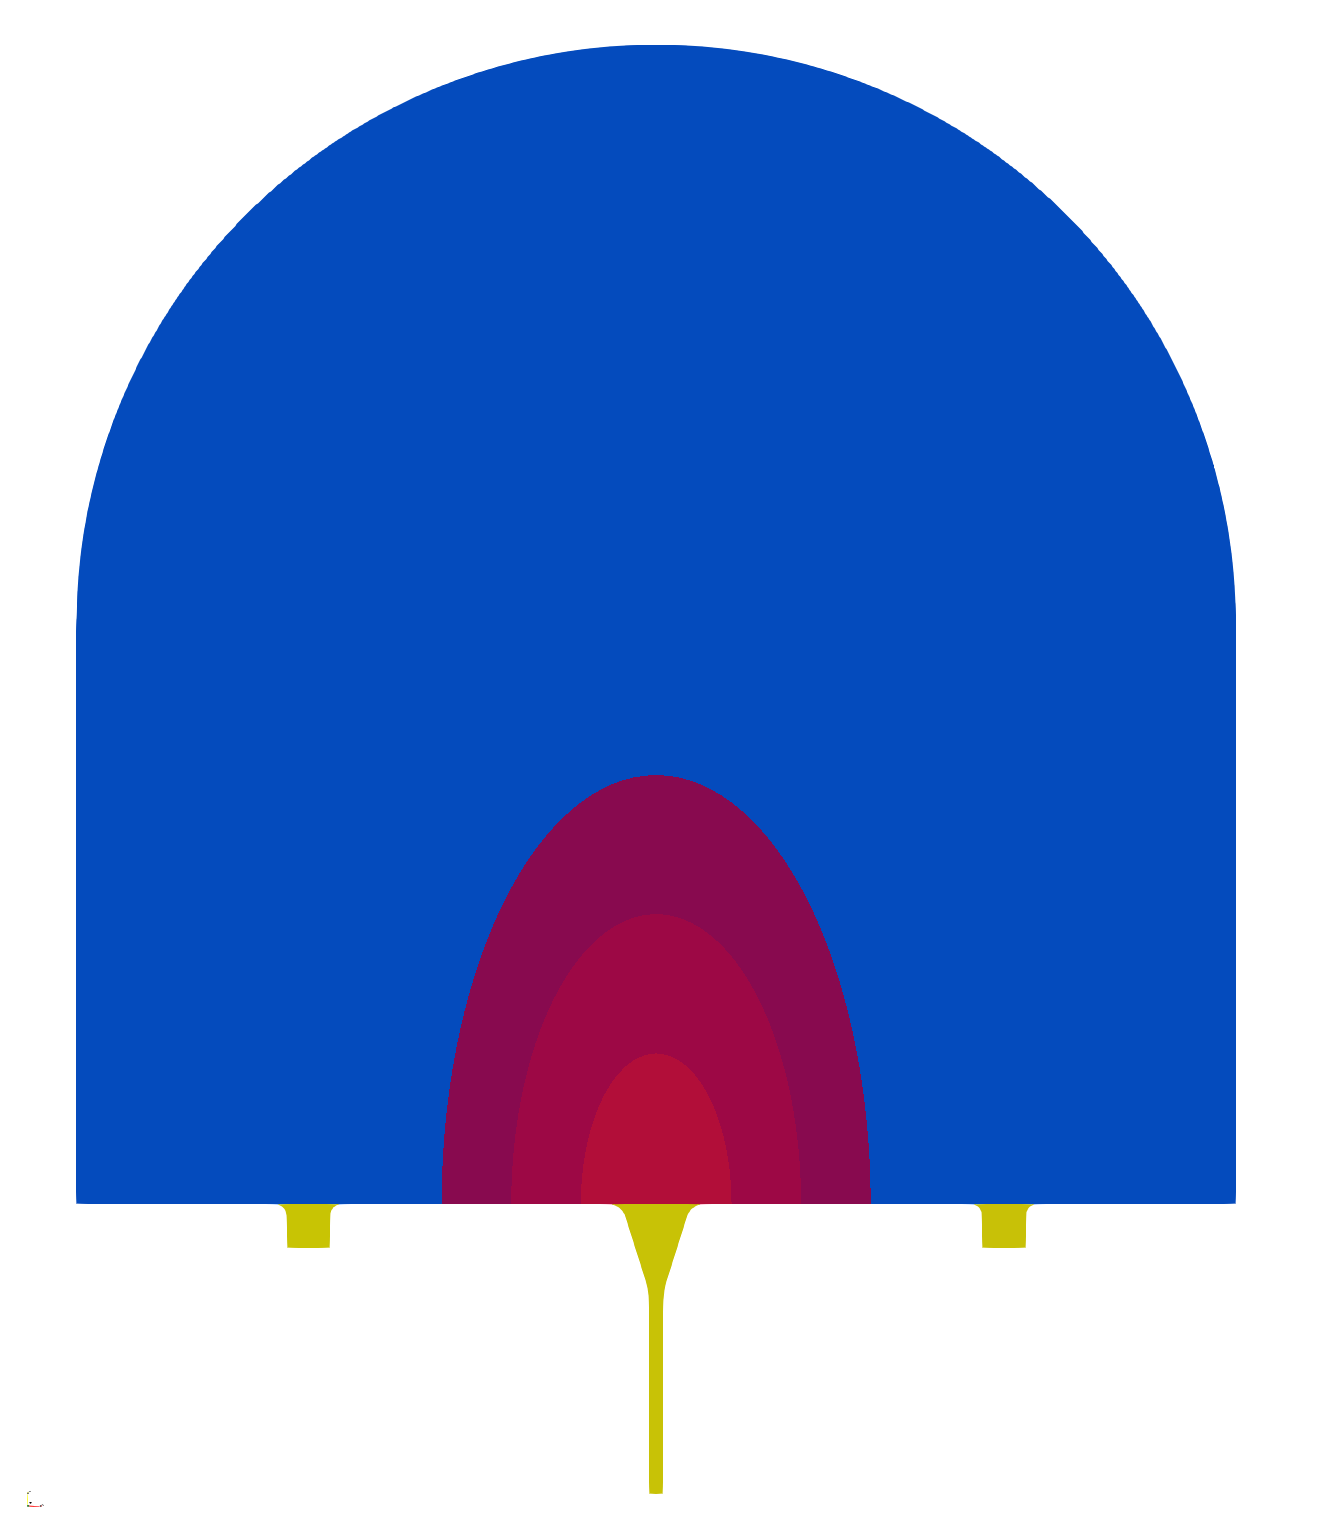
\includegraphics[width=190.54pt,height=218.28pt]{diagrams/placenta-geometry-diagrams/region_box-circle.png}};
%Shape: Rectangle [id:dp11952109232655417] 
\draw   (276.25,144.5) -- (368.5,144.5) -- (368.5,290) -- (276.25,290) -- cycle ;
%Shape: Polygon [id:ds32462111988530795] 
\draw  [fill={rgb, 255:red, 155; green, 155; blue, 155 }  ,fill opacity=0.2 ] (472.75,274.75) -- (368.5,290) -- (368.5,144.5) -- (472.75,47.5) -- cycle ;
%Shape: Rectangle [id:dp5451664654875743] 
\draw  [color={rgb, 255:red, 208; green, 2; blue, 27 }  ,draw opacity=1 ][fill={rgb, 255:red, 255; green, 255; blue, 255 }  ,fill opacity=1 ][line width=2.25] [blur shadow={shadow xshift=0pt,shadow yshift=0pt, shadow blur radius=1.5pt, shadow blur steps=4 ,shadow opacity=100}] (472.75,47.5) -- (628,47.5) -- (628,274.75) -- (472.75,274.75) -- cycle ;
%Shape: Rectangle [id:dp6890601408304888] 
\draw   (246.5,229) -- (266,229) -- (266,247) -- (246.5,247) -- cycle ;
%Shape: Polygon [id:ds42099539199351566] 
\draw  [fill={rgb, 255:red, 155; green, 155; blue, 155 }  ,fill opacity=0.2 ] (246.5,229) -- (246.5,247) -- (171,163.25) -- (171,49.5) -- cycle ;
%Shape: Rectangle [id:dp12209853757269817] 
\draw  [color={rgb, 255:red, 74; green, 144; blue, 226 }  ,draw opacity=1 ][fill={rgb, 255:red, 255; green, 255; blue, 255 }  ,fill opacity=1 ][line width=2.25] [blur shadow={shadow xshift=0pt,shadow yshift=0pt, shadow blur radius=1.5pt, shadow blur steps=4 ,shadow opacity=100}] (31,49.5) -- (171,49.5) -- (171,163.25) -- (31,163.25) -- cycle ;
%Shape: Axis 2D [id:dp5452843462335768] 
\draw  (143.68,262.48) -- (176.48,262.48)(146.96,232.96) -- (146.96,265.76) (169.48,257.48) -- (176.48,262.48) -- (169.48,267.48) (141.96,239.96) -- (146.96,232.96) -- (151.96,239.96)  ;

%Image [id:dp5542528854088136] 
\draw (550,147.64) node  {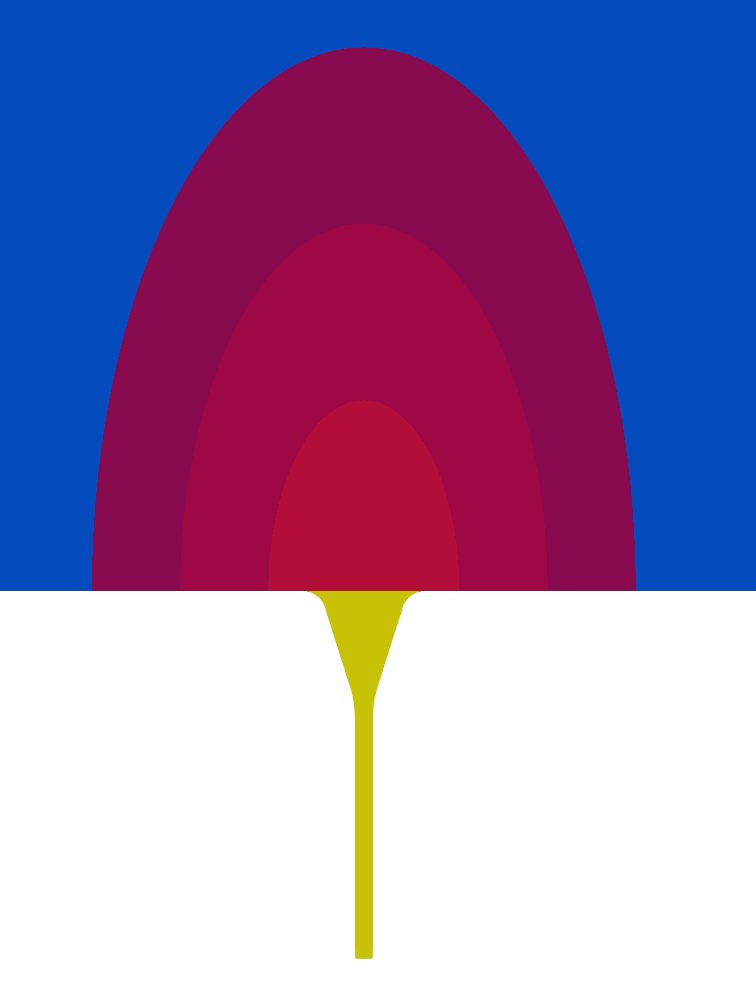
\includegraphics[width=107.25pt,height=141.58pt]{diagrams/placenta-geometry-diagrams/region_box-circle_artery.png}};
%Image [id:dp4703221885051676] 
\draw (101.5,97.38) node  {
\includegraphics[width=96.75pt,height=65.06pt]{diagrams/placenta-geometry-diagrams/region_box-circle_vein.png}};
%Shape: Arc [id:dp15907837716166395] 
\draw  [draw opacity=0][line width=3.75]  (514.1,164.59) .. controls (514.1,164.5) and (514.1,164.42) .. (514.1,164.34) .. controls (514.1,126.41) and (529.36,95.67) .. (548.18,95.67) .. controls (567,95.67) and (582.25,126.41) .. (582.25,164.34) .. controls (582.25,164.46) and (582.25,164.59) .. (582.25,164.72) -- (548.18,164.34) -- cycle ; \draw  [line width=3.75]  (514.1,164.59) .. controls (514.1,164.5) and (514.1,164.42) .. (514.1,164.34) .. controls (514.1,126.41) and (529.36,95.67) .. (548.18,95.67) .. controls (567,95.67) and (582.25,126.41) .. (582.25,164.34) .. controls (582.25,164.46) and (582.25,164.59) .. (582.25,164.72) ;  
%Straight Lines [id:da31968378407565723] 
\draw    (523,204.5) -- (541.48,192.62) ;
\draw [shift={(544,191)}, rotate = 147.26] [fill={rgb, 255:red, 0; green, 0; blue, 0 }  ][line width=0.08]  [draw opacity=0] (8.93,-4.29) -- (0,0) -- (8.93,4.29) -- cycle    ;
%Straight Lines [id:da21169793883490962] 
\draw [color={rgb, 255:red, 74; green, 144; blue, 226 }  ,draw opacity=1 ][line width=3.75]    (120,122.25) -- (77.25,122.25) ;
%Straight Lines [id:da48410947011907224] 
\draw [color={rgb, 255:red, 208; green, 2; blue, 27 }  ,draw opacity=1 ][line width=2.25]    (549,233.5) -- (545.75,233.5) ;
%Straight Lines [id:da8968866603549419] 
\draw [color={rgb, 255:red, 178; green, 15; blue, 57 }  ,draw opacity=1 ]   (550.25,168.5) -- (595.5,168.5) ;
\draw [shift={(598.5,168.5)}, rotate = 180] [fill={rgb, 255:red, 178; green, 15; blue, 57 }  ,fill opacity=1 ][line width=0.08]  [draw opacity=0] (5.36,-2.57) -- (0,0) -- (5.36,2.57) -- cycle    ;
\draw [shift={(547.25,168.5)}, rotate = 0] [fill={rgb, 255:red, 178; green, 15; blue, 57 }  ,fill opacity=1 ][line width=0.08]  [draw opacity=0] (5.36,-2.57) -- (0,0) -- (5.36,2.57) -- cycle    ;
%Straight Lines [id:da31654998264540546] 
\draw [color={rgb, 255:red, 178; green, 15; blue, 57 }  ,draw opacity=1 ]   (550.5,176.5) -- (579.25,176.5) ;
\draw [shift={(582.25,176.5)}, rotate = 180] [fill={rgb, 255:red, 178; green, 15; blue, 57 }  ,fill opacity=1 ][line width=0.08]  [draw opacity=0] (5.36,-2.57) -- (0,0) -- (5.36,2.57) -- cycle    ;
\draw [shift={(547.5,176.5)}, rotate = 0] [fill={rgb, 255:red, 178; green, 15; blue, 57 }  ,fill opacity=1 ][line width=0.08]  [draw opacity=0] (5.36,-2.57) -- (0,0) -- (5.36,2.57) -- cycle    ;
%Straight Lines [id:da2804690215211083] 
\draw [color={rgb, 255:red, 178; green, 15; blue, 57 }  ,draw opacity=1 ]   (551.5,184.25) -- (562,184.25) ;
\draw [shift={(565,184.25)}, rotate = 180] [fill={rgb, 255:red, 178; green, 15; blue, 57 }  ,fill opacity=1 ][line width=0.08]  [draw opacity=0] (5.36,-2.57) -- (0,0) -- (5.36,2.57) -- cycle    ;
\draw [shift={(548.5,184.25)}, rotate = 0] [fill={rgb, 255:red, 178; green, 15; blue, 57 }  ,fill opacity=1 ][line width=0.08]  [draw opacity=0] (5.36,-2.57) -- (0,0) -- (5.36,2.57) -- cycle    ;
%Straight Lines [id:da2427007571257227] 
\draw [color={rgb, 255:red, 155; green, 155; blue, 155 }  ,draw opacity=1 ] [dash pattern={on 0.84pt off 2.51pt}]  (565,166) -- (565,184.25) ;
%Straight Lines [id:da6267655040295248] 
\draw [color={rgb, 255:red, 155; green, 155; blue, 155 }  ,draw opacity=1 ] [dash pattern={on 0.84pt off 2.51pt}]  (582.25,164.72) -- (582.25,176.75) ;
%Straight Lines [id:da38228961483549484] 
\draw [color={rgb, 255:red, 0; green, 0; blue, 0 }  ,draw opacity=1 ] [dash pattern={on 0.84pt off 2.51pt}]  (119,106.9) -- (77.67,106.9) ;
%Straight Lines [id:da182869504277962] 
\draw [color={rgb, 255:red, 178; green, 15; blue, 57 }  ,draw opacity=1 ]   (65.83,84.1) -- (65.83,102.67) ;
\draw [shift={(65.83,105.67)}, rotate = 270] [fill={rgb, 255:red, 178; green, 15; blue, 57 }  ,fill opacity=1 ][line width=0.08]  [draw opacity=0] (5.36,-2.57) -- (0,0) -- (5.36,2.57) -- cycle    ;
\draw [shift={(65.83,81.1)}, rotate = 90] [fill={rgb, 255:red, 178; green, 15; blue, 57 }  ,fill opacity=1 ][line width=0.08]  [draw opacity=0] (5.36,-2.57) -- (0,0) -- (5.36,2.57) -- cycle    ;
%Straight Lines [id:da6948815579213783] 
\draw [color={rgb, 255:red, 128; green, 128; blue, 128 }  ,draw opacity=1 ] [dash pattern={on 0.84pt off 2.51pt}]  (119.33,98.05) -- (77.45,98.05) ;
%Straight Lines [id:da547314772003725] 
\draw [color={rgb, 255:red, 128; green, 128; blue, 128 }  ,draw opacity=1 ] [dash pattern={on 0.84pt off 2.51pt}]  (119,88.47) -- (77.38,88.47) ;
%Straight Lines [id:da8083416036570497] 
\draw    (134.67,119.02) -- (124.92,116.69) ;
\draw [shift={(122,116)}, rotate = 13.39] [fill={rgb, 255:red, 0; green, 0; blue, 0 }  ][line width=0.08]  [draw opacity=0] (5.36,-2.57) -- (0,0) -- (5.36,2.57) -- cycle    ;

% Text Node
\draw (179.86,259) node [anchor=west] [inner sep=0.75pt]  [font=\footnotesize]  {$x$};
% Text Node
\draw (148,226.55) node [anchor=south] [inner sep=0.75pt]  [font=\footnotesize]  {$y$};
% Text Node
\draw (133.57,114.07) node [anchor=north west][inner sep=0.75pt]  [font=\Large,color={rgb, 255:red, 0; green, 0; blue, 0 }  ,opacity=1 ]  {$\Omega _{\text{v}}$};
% Text Node
\draw (101.21,65.91) node  [font=\normalsize,color={rgb, 255:red, 255; green, 255; blue, 255 }  ,opacity=1 ]  {$\Omega _{\text{IVS}}$};
% Text Node
\draw (547.79,150.91) node  [font=\small,color={rgb, 255:red, 255; green, 255; blue, 255 }  ,opacity=1 ]  {$\Omega _{\text{CC}}$};
% Text Node
\draw (598.79,69.25) node  [font=\large,color={rgb, 255:red, 255; green, 255; blue, 255 }  ,opacity=1 ]  {$\Omega _{\text{IVS}}$};
% Text Node
\draw (524.5,200.4) node [anchor=north east] [inner sep=0.75pt]  [font=\LARGE,color={rgb, 255:red, 0; green, 0; blue, 0 }  ,opacity=1 ]  {$\Omega _{\text{a}}$};
% Text Node
\draw (323.38,90.08) node  [font=\LARGE,color={rgb, 255:red, 255; green, 255; blue, 255 }  ,opacity=1 ]  {$\Omega _{\text{IVS}}$};
% Text Node
\draw (99.38,127.2) node [anchor=north] [inner sep=0.75pt]  [font=\Large,color={rgb, 255:red, 74; green, 144; blue, 226 }  ,opacity=1 ]  {$\Gamma _{\text{out}}$};
% Text Node
\draw (547.5,237.7) node [anchor=north] [inner sep=0.75pt]  [font=\Large,color={rgb, 255:red, 208; green, 2; blue, 27 }  ,opacity=1 ]  {$\Gamma _{\text{in}}$};
% Text Node
\draw (557.54,187.4) node [anchor=north] [inner sep=0.75pt]  [font=\small,color={rgb, 255:red, 178; green, 15; blue, 57 }  ,opacity=1 ]  {$s_{0}$};
% Text Node
\draw (574.29,179.65) node [anchor=north] [inner sep=0.75pt]  [font=\small,color={rgb, 255:red, 178; green, 15; blue, 57 }  ,opacity=1 ]  {$s_{1}$};
% Text Node
\draw (590.79,171.4) node [anchor=north] [inner sep=0.75pt]  [font=\small,color={rgb, 255:red, 178; green, 15; blue, 57 }  ,opacity=1 ]  {$s_{2}$};
% Text Node
\draw (550.29,118.41) node  [font=\small,color={rgb, 255:red, 255; green, 255; blue, 255 }  ,opacity=1 ]  {$\Omega {_{\text{T}^{-}}^{\ }}^{\ }$};
% Text Node
\draw (549.79,78.41) node  [font=\small,color={rgb, 255:red, 255; green, 255; blue, 255 }  ,opacity=1 ]  {$\Omega {_{\text{T}^{+}}^{\ }}^{\ }$};
% Text Node
\draw (62.07,92.59) node [anchor=east] [inner sep=0.75pt]  [font=\scriptsize,color={rgb, 255:red, 0; green, 0; blue, 0 }  ,opacity=1 ]  {$\textcolor[rgb]{0.64,0.04,0.26}{y}\textcolor[rgb]{0.64,0.04,0.26}{_{0}}$};


\end{tikzpicture}
